% !BIB program = bibtex
\documentclass[12pt,a4paper,oneside]{report}

\def\TemplateMainLanguage{french}
% Start here: your details and the on/off switches.
% Help: https://github.com/KaiyuanGONG/lmfi-thesis-template

\newcommand{\ThesisTitleEN}{Reachability in Finite Directed Graphs}
\newcommand{\ThesisTitleFR}{Accessibilité dans les graphes orientés finis}
\newcommand{\ThesisAuthor}{Student Name}
\newcommand{\ThesisInstitution}{Université Paris Cité}
\newcommand{\ThesisProgramme}{M2 Logique Mathématique et Fondements de l'Informatique (LMFI)}
\newcommand{\ThesisSupervisors}{Supervisor Name\\Co-supervisor Name}
% Optional academic referent (enseignant référent); leave empty to omit the line.
\newcommand{\ThesisReferent}{Referent Name}
\newcommand{\ThesisLaboratory}{}
\newcommand{\ThesisLocation}{Paris}
\newcommand{\ThesisAcademicYear}{2026--2027}
\newcommand{\ThesisDateEN}{September 2027}
\newcommand{\ThesisDateFR}{septembre 2027}
\newcommand{\ThesisKeywordsEN}{directed graph, reachability, transitive closure}
\newcommand{\ThesisKeywordsFR}{graphe orienté, accessibilité, clôture transitive}

% Title-page logos (left, centre, right): a file path, empty for a grey box,
% or none. No logo is included; use only files you are allowed to use.
\newcommand{\ThesisLogoFile}{}
\newcommand{\ThesisLogoFileTwo}{}
\newcommand{\ThesisLogoFileThree}{}

% On/off switches. To leave a part out, change true to false.
% Abstract in the other language (French résumé or English abstract):
\newif\ifincludesecondaryabstract
\includesecondaryabstracttrue
% Acknowledgements page:
\newif\ifincludeacknowledgements
\includeacknowledgementstrue
% Lists of figures and of tables, after the contents:
\newif\ifincludelistoffigures
\includelistoffiguresfalse
\newif\ifincludelistoftables
\includelistoftablesfalse
% Appendices (the appendices/ folder):
\newif\ifincludeappendix
\includeappendixtrue
% LaTeX examples (figures, tables, code, ...) as Appendices B and C. Change to
% true to see them, and back to false before submitting.
\newif\ifincludeexamples
\includeexamplesfalse

% Shared preamble for main.tex and main-fr.tex.

% Encoding and languages
\usepackage[utf8]{inputenc}
\usepackage[T1]{fontenc}
% Numeric citations in order of appearance ([1], [2], ...), processed by BibTeX.
% natbib must be loaded before babel-french.
\usepackage[numbers,sort&compress]{natbib}
% The main language must be the document language: babel-french restyles
% lists and footnotes only when French is the main language.
\usepackage[main=\TemplateMainLanguage,english,french]{babel}
\usepackage{csquotes}
\usepackage{etoolbox}

% Page and paragraph layout
\usepackage[a4paper,left=3cm,right=2.5cm,top=3cm,bottom=3cm]{geometry}
\setlength{\parindent}{0pt}
\setlength{\parskip}{0.55em}
\renewcommand{\baselinestretch}{1.08}

% Mathematics and fonts: amsmath must precede newtxmath.
\usepackage{amsmath}
\usepackage{mathtools}
\usepackage{amsthm}
\usepackage{libertine}
\usepackage[libertine]{newtxmath}

% Figures, tables, algorithms
\usepackage{graphicx}
\usepackage{booktabs}
\usepackage{array}
\usepackage{tabularx}
\usepackage{longtable}
\usepackage[labelsep=endash]{caption}
\usepackage{subcaption}
\usepackage{pdflscape}
\usepackage{tikz}
\usetikzlibrary{arrows.meta,positioning}
\usepackage{tikz-cd}
\usepackage{mathpartir}
\usepackage{algorithm}
\usepackage{algpseudocode}
\usepackage{listings}

% Typographic polish
\usepackage{microtype}
\usepackage{xcolor}
\usepackage{fancyhdr}
\usepackage{siunitx}
\usepackage{acro}

\definecolor{LMFINavy}{HTML}{304B8A}
\definecolor{LMFITeal}{HTML}{0F766E}

% Portable code examples: listings needs no shell escape or external program.
\lstdefinestyle{TemplateCode}{
  basicstyle=\ttfamily\small,
  keywordstyle=\color{LMFINavy}\bfseries,
  commentstyle=\color{LMFITeal},
  numbers=left,
  numberstyle=\tiny\color{gray},
  numbersep=8pt,
  frame=lines,
  rulecolor=\color{LMFINavy},
  breaklines=true,
  showstringspaces=false,
  tabsize=2,
  captionpos=b
}

% Localised strings and selected metadata
\ifdefstring{\TemplateMainLanguage}{french}{%
  % babel-french normally activates :;!? to insert spaces. Active colons also
  % enter label keys such as ch:background and break cleveref. French source in
  % this template writes the required spaces explicitly, so keep punctuation
  % inactive and labels portable.
  \frenchsetup{AutoSpacePunctuation=false}
  \newcommand{\TemplateTitle}{\ThesisTitleFR}
  \newcommand{\TemplateDate}{\ThesisDateFR}
  \newcommand{\TemplateKeywords}{\ThesisKeywordsFR}
  \newcommand{\TemplatePdfLang}{fr-FR}
  \newcommand{\TemplateThesisType}{Mémoire de master}
  \newcommand{\TemplateSupervisionLabel}{Sous la direction de}
  \newcommand{\TemplateLaboratoryLabel}{Laboratoire d'accueil}
  \newcommand{\TemplateAcademicYearLabel}{Année universitaire}
  \newcommand{\TemplateLogoLabel}{Logo institutionnel facultatif}
  \newcommand{\TemplateReferentLabel}{Enseignant référent}
  \newcommand{\TemplateReferencesTitle}{Références}
  \bibliographystyle{unsrtnat-fr}
  \newcommand{\theoremname}{Théorème}
  \newcommand{\propositionname}{Proposition}
  \newcommand{\lemmaname}{Lemme}
  \newcommand{\corollaryname}{Corollaire}
  \newcommand{\assumptionname}{Hypothèse}
  \newcommand{\definitionname}{Définition}
  \newcommand{\examplename}{Exemple}
  \newcommand{\remarkname}{Remarque}
  \floatname{algorithm}{Algorithme}
  % babel-french names table captions "Table"; French theses write "Tableau".
  \addto\captionsfrench{\renewcommand{\tablename}{Tableau}}
  \renewcommand{\lstlistingname}{Extrait de code}
  \renewcommand{\lstlistlistingname}{Liste des extraits de code}
  \algrenewcommand\algorithmicrequire{\textbf{Entrée :}}
  \algrenewcommand\algorithmicensure{\textbf{Sortie :}}
  \algrenewcommand\algorithmicreturn{\textbf{retourner}}
  \algrenewcommand\algorithmicfor{\textbf{pour}}
  \algrenewcommand\algorithmicdo{\textbf{faire}}
  \algrenewcommand\algorithmicend{\textbf{fin}}
}{%
  \newcommand{\TemplateTitle}{\ThesisTitleEN}
  \newcommand{\TemplateDate}{\ThesisDateEN}
  \newcommand{\TemplateKeywords}{\ThesisKeywordsEN}
  \newcommand{\TemplatePdfLang}{en-GB}
  \newcommand{\TemplateThesisType}{Master's thesis}
  \newcommand{\TemplateSupervisionLabel}{Supervised by}
  \newcommand{\TemplateLaboratoryLabel}{Host laboratory}
  \newcommand{\TemplateAcademicYearLabel}{Academic year}
  \newcommand{\TemplateLogoLabel}{Optional institutional logo}
  \newcommand{\TemplateReferentLabel}{Academic referent}
  \newcommand{\TemplateReferencesTitle}{References}
  \bibliographystyle{unsrtnat}
  \newcommand{\theoremname}{Theorem}
  \newcommand{\propositionname}{Proposition}
  \newcommand{\lemmaname}{Lemma}
  \newcommand{\corollaryname}{Corollary}
  \newcommand{\assumptionname}{Assumption}
  \newcommand{\definitionname}{Definition}
  \newcommand{\examplename}{Example}
  \newcommand{\remarkname}{Remark}
  \floatname{algorithm}{Algorithm}
  \renewcommand{\lstlistingname}{Code listing}
  \renewcommand{\lstlistlistingname}{List of code listings}
  \algrenewcommand\algorithmicrequire{\textbf{Input:}}
  \algrenewcommand\algorithmicensure{\textbf{Output:}}
  \algrenewcommand\algorithmicreturn{\textbf{return}}
}

% Labels follow the language in force, so an abstract in the secondary language
% is labelled in that language. The French keyword label carries its own
% non-breaking space before the colon.
\newcommand{\TemplateKeywordsLabel}{\iflanguage{french}{Mots-clés~:}{Keywords:}}

% Float placement: pack floats from the top of a float page and let a page hold
% more float and less forced text, which avoids loose float pages.
\makeatletter
\setlength{\@fptop}{0pt}
\setlength{\@fpsep}{14pt}
\setlength{\@fpbot}{0pt plus 1fil}
\makeatother
\renewcommand{\topfraction}{0.95}
\renewcommand{\bottomfraction}{0.95}
\renewcommand{\textfraction}{0.06}
\renewcommand{\floatpagefraction}{0.80}
\setlength{\textfloatsep}{16pt plus 3pt minus 3pt}
\setlength{\floatsep}{14pt plus 3pt minus 3pt}
% A little extra stretch for lines that carry long inline formulas.
\setlength{\emergencystretch}{3em}

% Headers: chapter title on the right, page number centred in the footer.
\pagestyle{fancy}
\setlength{\headheight}{14.5pt}
\fancyhf{}
\fancyhead[R]{\small\nouppercase{\leftmark}}
\fancyfoot[C]{\thepage}
\renewcommand{\headrulewidth}{0.4pt}
\renewcommand{\footrulewidth}{0pt}
\fancypagestyle{plain}{%
  \fancyhf{}
  \fancyfoot[C]{\thepage}
  \renewcommand{\headrulewidth}{0pt}}

% The bibliography is an unnumbered chapter listed in the table of contents.
\renewcommand{\bibsection}{%
  \chapter*{\TemplateReferencesTitle}%
  \phantomsection\addcontentsline{toc}{chapter}{\TemplateReferencesTitle}%
  \markboth{\TemplateReferencesTitle}{\TemplateReferencesTitle}}

% Links are clickable but not coloured, so the PDF prints cleanly.
\usepackage[hidelinks,unicode=true]{hyperref}
\usepackage[capitalise,noabbrev]{cleveref}

% Theorem-like environments are defined after cleveref is loaded: cleveref must
% see them in order to name shared-counter environments correctly.
% Theorem environments share one counter, numbered within chapters
% (Theorem 3.2); equations follow the same scheme, e.g. (3.1).
\theoremstyle{plain}
\newtheorem{theorem}{\theoremname}[chapter]
\newtheorem{proposition}[theorem]{\propositionname}
\newtheorem{lemma}[theorem]{\lemmaname}
\newtheorem{corollary}[theorem]{\corollaryname}

\theoremstyle{definition}
\newtheorem{definition}[theorem]{\definitionname}
\newtheorem{assumption}[theorem]{\assumptionname}
\newtheorem{example}[theorem]{\examplename}

\theoremstyle{remark}
\newtheorem{remark}[theorem]{\remarkname}

\numberwithin{equation}{chapter}

\ifdefstring{\TemplateMainLanguage}{french}{%
  \crefname{chapter}{chapitre}{chapitres}
  \crefname{section}{section}{sections}
  \crefname{figure}{figure}{figures}
  \crefname{table}{tableau}{tableaux}
  \crefname{algorithm}{algorithme}{algorithmes}
  \crefname{theorem}{théorème}{théorèmes}
  \crefname{lemma}{lemme}{lemmes}
  \crefname{corollary}{corollaire}{corollaires}
  \crefname{assumption}{hypothèse}{hypothèses}
  \crefname{example}{exemple}{exemples}
  \crefname{remark}{remarque}{remarques}
  \crefname{proposition}{proposition}{propositions}
  \crefname{definition}{définition}{définitions}
  \crefname{equation}{équation}{équations}
  \crefname{listing}{extrait de code}{extraits de code}
  \Crefname{listing}{Extrait de code}{Extraits de code}
  \providecommand{\crefpairconjunction}{}
  \providecommand{\creflastconjunction}{}
  \providecommand{\crefpairgroupconjunction}{}
  \providecommand{\creflastgroupconjunction}{}
  \renewcommand{\crefpairconjunction}{ et }
  \renewcommand{\creflastconjunction}{ et }
  \renewcommand{\crefpairgroupconjunction}{ et }
  \renewcommand{\creflastgroupconjunction}{ et }
}{%
  \crefname{chapter}{chapter}{chapters}
  \crefname{section}{section}{sections}
  \crefname{figure}{figure}{figures}
  \crefname{table}{table}{tables}
  \crefname{algorithm}{algorithm}{algorithms}
  \crefname{theorem}{theorem}{theorems}
  \crefname{lemma}{lemma}{lemmas}
  \crefname{corollary}{corollary}{corollaries}
  \crefname{assumption}{assumption}{assumptions}
  \crefname{example}{example}{examples}
  \crefname{remark}{remark}{remarks}
  \crefname{proposition}{proposition}{propositions}
  \crefname{definition}{definition}{definitions}
  \crefname{equation}{equation}{equations}
  \crefname{listing}{code listing}{code listings}
  \Crefname{listing}{Code listing}{Code listings}
}

% Number formatting follows the language of the thesis (1.5 or 1,5).
\ifdefstring{\TemplateMainLanguage}{french}{\sisetup{locale=FR}}{\sisetup{locale=UK}}

% Project macros and abbreviations (edit macros.tex, not this file).
% Project macros and abbreviations, loaded by preamble.tex.
% Keep notation that you reuse here; delete anything the thesis does not use.

% Sets and operators
\newcommand{\N}{\mathbb{N}}
\DeclareMathOperator{\Reach}{Reach}

% Semantic brackets. These two macros draw the usual double brackets without an
% extra font; stmaryrd provides true glyphs if you prefer them. \sem{\varphi}
% sets the argument, and \sem*{\varphi} resizes the brackets to fit it.
\providecommand{\llbracket}{\mathopen{[\mkern-3.3mu[}}
\providecommand{\rrbracket}{\mathclose{]\mkern-3.3mu]}}
\DeclarePairedDelimiter{\sem}{\llbracket}{\rrbracket}

% Abbreviations used by the acro package (\ac, \acs, \acf, \printacronyms).
% Give the long form in the language of the thesis.
\ifdefstring{\TemplateMainLanguage}{french}{%
  \DeclareAcronym{dag}{short = DAG, long = graphe orienté acyclique}
  \DeclareAcronym{scc}{short = CFC, long = composante fortement connexe}
}{%
  \DeclareAcronym{dag}{short = DAG, long = directed acyclic graph}
  \DeclareAcronym{scc}{short = SCC, long = strongly connected component}
}


\hypersetup{
  pdftitle={\TemplateTitle},
  pdfauthor={\ThesisAuthor},
  pdfsubject={\ThesisProgramme},
  pdfkeywords={\TemplateKeywords},
  pdflang={\TemplatePdfLang}
}

\newcommand{\TemplateActivateLanguage}{%
  \selectlanguage{\TemplateMainLanguage}%
  \ifdefstring{\TemplateMainLanguage}{french}{\shorthandoff{:}}{}%
}
\AtBeginDocument{\TemplateActivateLanguage}


% Pendant la rédaction, décommentez une sélection pour ne compiler que ces chapitres.
% \includeonly{chapters/fr/03-main-work,chapters/fr/04-applications-evaluation}

\begin{document}
\TemplateActivateLanguage

% Les ancres sont désactivées sur la couverture afin d'éviter les doublons PDF.
\hypersetup{pageanchor=false}
\pagenumbering{gobble}
% Neutral logo box, shown when a logo slot is empty or its file is missing.
\newcommand{\TemplateLogoPlaceholder}{%
  \fcolorbox{LMFINavy}{white}{%
    \parbox[c][1.35cm][c]{0.88\linewidth}{%
      \centering\small\textcolor{LMFINavy}{\TemplateLogoLabel}}}}

% #1 is a metadata macro holding a file path. An empty path shows the neutral
% box and the value none leaves the slot blank.
\newcommand{\TemplateLogoSlot}[1]{%
  \ifdefempty{#1}{%
    \TemplateLogoPlaceholder
  }{%
    \ifdefstring{#1}{none}{}{%
      \IfFileExists{#1}{%
        \includegraphics[height=1.35cm,width=\linewidth,keepaspectratio]{#1}%
      }{%
        \PackageWarning{lmfi-template}{Logo file `#1' not found; using placeholder}%
        \TemplateLogoPlaceholder
      }%
    }%
  }%
}

\begin{titlepage}
  \thispagestyle{empty}

  \noindent
  \begin{minipage}[c][2.3cm][c]{0.31\textwidth}
    \raggedright\TemplateLogoSlot{\ThesisLogoFile}%
  \end{minipage}%
  \hfill
  \begin{minipage}[c][2.3cm][c]{0.31\textwidth}
    \centering\TemplateLogoSlot{\ThesisLogoFileTwo}%
  \end{minipage}%
  \hfill
  \begin{minipage}[c][2.3cm][c]{0.31\textwidth}
    \raggedleft\TemplateLogoSlot{\ThesisLogoFileThree}%
  \end{minipage}

  \vfill

  \begin{center}
    {\color{LMFINavy}\rule{\linewidth}{0.7mm}}\\[0.45cm]
    {\Large\bfseries\TemplateTitle\par}
    \vspace{0.45cm}
    {\color{LMFINavy}\rule{\linewidth}{0.3mm}}
  \end{center}

  \vfill

  \begin{center}
    {\Large\textsc{\ThesisAuthor}}\\[1.2cm]

    \textbf{\TemplateSupervisionLabel}\\[0.35cm]
    \ThesisSupervisors%
    \ifdefempty{\ThesisReferent}{}{%
      \\[0.9cm]
      \textbf{\TemplateReferentLabel}\\[0.25cm]
      \ThesisReferent}%
    \ifdefempty{\ThesisLaboratory}{}{%
      \\[0.9cm]
      \textbf{\TemplateLaboratoryLabel}\\[0.25cm]
      \ThesisLaboratory}
  \end{center}

  \vfill

  \begin{center}
    \TemplateThesisType\\
    \ThesisProgramme\\
    \ThesisInstitution\\[0.8cm]
    \TemplateAcademicYearLabel{} \ThesisAcademicYear\\
    \ThesisLocation, \TemplateDate
  \end{center}
\end{titlepage}

\clearpage

\hypersetup{pageanchor=true}
\pagenumbering{roman}
\setcounter{page}{1}
\begin{otherlanguage}{french}
\chapter*{Résumé}
\addcontentsline{toc}{chapter}{Résumé}
\markboth{Résumé}{Résumé}

% Remplacez cette page par une présentation concise de la question, de la
% méthode, du résultat principal et des limites. Le résumé doit pouvoir être
% lu indépendamment du mémoire et ne doit pas annoncer de résultat absent du
% texte.

Ce mémoire miniature étudie l'accessibilité dans les graphes orientés finis. Il
introduit la clôture transitive de la relation d'arêtes, démontre une propriété
structurelle élémentaire et présente un algorithme matriciel qui calcule toutes
les paires accessibles. Un exemple à quatre sommets relie les définitions, la
figure, le tableau et l'algorithme utilisés pour illustrer le modèle. Cet exemple
reste volontairement court : il montre une méthode de travail cohérente en
LaTeX, sans imposer le contenu ni la longueur d'un mémoire LMFI.

\medskip
\noindent\textbf{\TemplateKeywordsLabel} \ThesisKeywordsFR
\end{otherlanguage}

\ifincludesecondaryabstract
  \begin{otherlanguage}{english}
\chapter*{Abstract}
\addcontentsline{toc}{chapter}{Abstract}
\markboth{Abstract}{Abstract}

% Replace this page with a concise account of the question, method, main
% result, and limitations. The abstract should stand on its own and should not
% introduce claims that are absent from the thesis.

This miniature thesis studies reachability in finite directed graphs. It introduces
the transitive closure of an edge relation, proves a basic structural property, and
presents a matrix algorithm that computes all reachable pairs. A four-vertex
example connects the formal definitions, algorithm, figure, and table used to
demonstrate the template. The example is intentionally small: its purpose is to
show a coherent LaTeX workflow, not to prescribe the content or length of an LMFI
thesis.

\medskip
\noindent\textbf{\TemplateKeywordsLabel} \ThesisKeywordsEN
\end{otherlanguage}

\fi
\ifincludeacknowledgements
  \chapter*{Remerciements}
\addcontentsline{toc}{chapter}{Remerciements}
\markboth{Remerciements}{Remerciements}

% Cette page est facultative : pour la retirer, remplacez
% \includeacknowledgementstrue par \includeacknowledgementsfalse dans
% metadata.tex. Remerciez uniquement les personnes ou organismes ayant
% réellement contribué au travail et vérifiez avec votre encadrant avant de
% nommer un partenaire soumis à confidentialité.

Je remercie mes encadrants pour leurs conseils et leur relecture attentive de ce
mémoire, ainsi que les membres du laboratoire d'accueil pour leur accueil
pendant le stage. Je remercie également l'équipe pédagogique du master, ainsi
que ma famille et mes amis pour leur soutien.

\fi

\clearpage\phantomsection\addcontentsline{toc}{chapter}{\contentsname}
{\renewcommand{\baselinestretch}{1}\setlength{\parskip}{0pt}\selectfont\tableofcontents}
\ifincludelistoffigures
  \listoffigures
\fi
\ifincludelistoftables
  \listoftables
\fi
\clearpage

\pagenumbering{arabic}
\setcounter{page}{1}
\chapter{Introduction}
\label{ch:introduction}

% Une introduction de mémoire présente généralement le contexte, la question
% précise, la contribution et un guide de lecture. Pour un rapport long,
% quatre à six pages suffisent souvent ; il s'agit d'un conseil de
% planification et non d'une règle LMFI.

Les graphes orientés modélisent des relations à sens unique : une dépendance peut
relier une tâche à une autre, ou une transition peut conduire d'un état de
programme à son successeur. Une première question consiste à déterminer si un
sommet est accessible depuis un autre en suivant zéro ou plusieurs arêtes. Ce
problème élémentaire relie ici définitions mathématiques, démonstrations,
algorithmes, figures, tableaux et références dans un même exemple. Des
introductions classiques figurent notamment dans \cite{diestel2017,cormen2022}.

\section{Question et contribution}

L'exemple répond à la question suivante : comment définir l'accessibilité dans
un graphe orienté fini, démontrer sa transitivité et la calculer à partir d'une
matrice d'adjacence ? La contribution reste volontairement modeste. Nous
formalisons la relation au \cref{ch:background}, la calculons au
\cref{ch:main-work} et étudions un cas concret au \cref{ch:evaluation}.

\section{Organisation de l'exemple}

La séparation entre préliminaires, travail principal et évaluation illustre une
structure de chapitres maintenable. Un mémoire théorique peut diviser le travail
principal en plusieurs chapitres de résultats ; un mémoire appliqué peut diviser
l'évaluation en protocole, résultats et discussion. Les fichiers sources rendent
ces deux adaptations locales et explicites.

\chapter{Contexte et préliminaires}
\label{ch:background}

% Introduisez uniquement les notations et résultats antérieurs utilisés
% ensuite. Indiquez clairement ce qui est classique et citez sa source ; ne
% transformez pas ce chapitre en panorama sans lien avec la suite.

\begin{definition}[Graphe orienté fini]
\label{def:directed-graph}
Un \emph{graphe orienté fini} est un couple $G=(V,E)$, où $V$ est un ensemble
fini de sommets et $E\subseteq V\times V$ un ensemble d'arêtes orientées.
\end{definition}

\begin{definition}[Accessibilité]
\label{def:reachability}
Soit $G=(V,E)$ un graphe orienté fini. Un sommet $v\in V$ est
\emph{accessible} depuis $u\in V$, ce que l'on note $u\mathrel{R^*}v$, s'il
existe un chemin de longueur $k\geq 0$ de $u$ vers $v$. Un chemin de longueur
nulle rend chaque sommet accessible depuis lui-même.
\end{definition}

En notant $R=E$ la relation d'arêtes et $I_V$ la relation identité sur $V$, la
clôture réflexive transitive est
\begin{equation}
  R^* = \bigcup_{k\geq 0} R^k,
  \label{eq:transitive-closure}
\end{equation}
où $R^0=I_V$ et les puissances de relations sont définies par composition. Cette
construction classique est présentée sous des angles complémentaires dans
\cite{diestel2017,cormen2022}.

\begin{theorem}[Transitivité de l'accessibilité]
\label{thm:transitivity}
Pour tous sommets $u,v,w\in V$, si $u\mathrel{R^*}v$ et
$v\mathrel{R^*}w$, alors $u\mathrel{R^*}w$.
\end{theorem}

\begin{proof}
La première hypothèse fournit un chemin de $u$ à $v$, et la seconde un chemin
de $v$ à $w$. Leur concaténation forme un chemin de $u$ à $w$. Ainsi,
$u\mathrel{R^*}w$ d'après la \cref{def:reachability}.
\end{proof}

Le \cref{thm:transitivity} découle aussi directement de
l'\cref{eq:transitive-closure} : l'union contient les chemins de toute longueur
finie et reste fermée par concaténation.

\begin{corollary}[L'accessibilité est un préordre]
\label{cor:preorder}
La relation $R^*$ est réflexive et transitive sur $V$ : la réflexivité vient des
chemins de longueur nulle (\cref{def:reachability}) et la transitivité est le
\cref{thm:transitivity}.
\end{corollary}

\chapter{Travail principal}
\label{ch:main-work}

% Ce chapitre constitue le cœur du mémoire. Remplacez le petit algorithme
% ci-dessous par la construction, la méthode ou la suite de théorèmes
% principale. Énoncez les hypothèses avant les résultats et justifiez chaque
% étape.

\begin{assumption}[Sommets indexés]
\label{ass:indexed-vertices}
$V=\{1,\dots,n\}$, et les arêtes sont données par une matrice booléenne
$A\in\{0,1\}^{n\times n}$.
\end{assumption}

Sous l'\cref{ass:indexed-vertices}, la méthode classique de Warshall \cite{warshall1962}
met à jour une matrice booléenne de sorte qu'après l'itération $k$, elle décrive
les chemins dont les sommets intermédiaires appartiennent à
$\{1,\dots,k\}$. Une version compacte est donnée par
l'\cref{alg:warshall}.

\begin{algorithm}[htbp]
\caption{Clôture réflexive transitive d'une matrice d'adjacence}
\label{alg:warshall}
\begin{algorithmic}[1]
  \Require matrice d'adjacence $A\in\{0,1\}^{n\times n}$
  \Ensure matrice d'accessibilité $T$
  \State $T\gets A\lor I_n$
  \For{$k\gets 1$ à $n$}
    \For{$i\gets 1$ à $n$}
      \For{$j\gets 1$ à $n$}
        \State $T_{ij}\gets T_{ij}\lor(T_{ik}\land T_{kj})$
      \EndFor
    \EndFor
  \EndFor
  \State \Return $T$
\end{algorithmic}
\end{algorithm}

\begin{proposition}
\label{prop:warshall-correct}
À la fin de l'\cref{alg:warshall}, $T_{ij}=1$ exactement lorsque $j$ est
accessible depuis $i$.
\end{proposition}

\begin{proof}
On raisonne par récurrence sur $k$. Initialement, $T$ décrit les chemins de
longueur zéro ou un. À l'itération $k$, la mise à jour ajoute précisément les
chemins qui passent par le sommet $k$ ; après la dernière itération, $T$
représente donc la relation de l'\cref{eq:transitive-closure}.
\end{proof}

\chapter{Applications, évaluation et discussion}
\label{ch:evaluation}

% Pour un travail théorique, utilisez ce chapitre pour les exemples,
% conséquences ou limites. Pour un travail empirique, séparez protocole,
% résultats et discussion.

Considérons le graphe de la \cref{fig:example-graph}. Ses arêtes directes sont
$a\to b$, $b\to c$, $c\to d$ et $a\to d$. La figure est dessinée avec TikZ :
elle reste nette quel que soit le zoom.

\begin{figure}[htbp]
  \centering
  \begin{tikzpicture}[
  vertex/.style={circle,draw=LMFINavy,thick,minimum size=8mm,inner sep=0pt},
  edge/.style={-{Stealth[length=2.4mm]},thick,LMFITeal},
  node distance=2.2cm
]
  \node[vertex] (a) {$a$};
  \node[vertex, right=of a] (b) {$b$};
  \node[vertex, right=of b] (c) {$c$};
  \node[vertex, below=1.0cm of c] (d) {$d$};

  \draw[edge] (a) -- (b);
  \draw[edge] (b) -- (c);
  \draw[edge] (c) -- (d);
  \draw[edge] (a) to[bend right=18] (d);
\end{tikzpicture}

  \caption{Graphe orienté à quatre sommets utilisé pour évaluer l'accessibilité.}
  \label{fig:example-graph}
\end{figure}

L'application de l'\cref{alg:warshall} donne la matrice réflexive d'accessibilité
du \cref{tab:reachability}. Le sommet $a$ atteint tous les sommets, tandis que
$d$ n'atteint que lui-même. L'entrée de la ligne $b$ et de la colonne $d$
représente le chemin $b\to c\to d$, bien qu'il n'existe pas d'arête directe
$b\to d$.

\begin{table}[htbp]
  \centering
  \caption{Matrice réflexive d'accessibilité de la \cref{fig:example-graph}.}
  \label{tab:reachability}
  \begin{tabular}{c *{4}{>{\centering\arraybackslash}p{1.2cm}}}
    \toprule
    De $\backslash$ vers & $a$ & $b$ & $c$ & $d$ \\
    \midrule
    $a$ & 1 & 1 & 1 & 1 \\
    $b$ & 0 & 1 & 1 & 1 \\
    $c$ & 0 & 0 & 1 & 1 \\
    $d$ & 0 & 0 & 0 & 1 \\
    \bottomrule
  \end{tabular}
\end{table}

Cet exemple vérifie la cohérence interne plutôt que la performance. Un véritable
chapitre expérimental doit préciser les données, la version du logiciel,
la métrique et l'incertitude, et discuter les cas négatifs : l'accessibilité
seule perd les longueurs de chemins.

\chapter{Conclusion}
\label{ch:conclusion}

% Répondez à la question posée dans l'introduction. Séparez résultats établis,
% limites et perspectives ; n'introduisez pas ici un nouveau théorème ou une
% nouvelle expérience.

Nous avons défini l'accessibilité comme la clôture réflexive transitive de
l'\cref{eq:transitive-closure}, démontré sa transitivité au
\cref{thm:transitivity} et calculé cette relation avec
l'\cref{alg:warshall}. Le graphe de la \cref{fig:example-graph} et la matrice du
\cref{tab:reachability} ont fourni une vérification transparente
des définitions et de l'algorithme.

L'exemple laisse volontairement ouvertes de nombreuses questions : reconstruction
des chemins, algorithmes pour graphes creux ou mises à jour incrémentales. Son
objectif principal reste structurel : montrer comment relier question de
recherche, définitions, résultats, preuves, limites et références correctement
citées, sans adopter une mise en page de type éditeur.


\bibliography{references}

\ifincludeappendix
  \appendix
  \chapter{Une courte trace matricielle}
\label{app:matrix-trace}

% Les annexes regroupent des éléments utiles qui interrompraient l'argument
% principal. Toute annexe doit être citée dans le mémoire. Pour retirer toutes
% les annexes, remplacez \includeappendixtrue par \includeappendixfalse dans
% metadata.tex.

Dans l'ordre $(a,b,c,d)$, la matrice booléenne initiale $A\lor I_4$ est
\[
\begin{pmatrix}
1&1&0&1\\
0&1&1&0\\
0&0&1&1\\
0&0&0&1
\end{pmatrix}.
\]
Lorsque $c$ devient un sommet intermédiaire autorisé, l'entrée $(b,d)$ passe de
zéro à un. Il s'agit du fait d'accessibilité non directe décrit sous le
\cref{tab:reachability}.

  \ifincludeexamples
    \chapter{Exemples LaTeX courants}
\label{app:latex-patterns}

% Cette annexe facultative est un aide-mémoire et ne fait pas partie de
% l'argument sur l'accessibilité. Ne conservez que les formes réellement
% utilisées, remplacez chaque ressource pédagogique et commentez dans le texte
% toute figure, tout tableau, toute équation ou tout extrait de code conservé.

\section{Illustration externe}

Le projet contient le fichier vectoriel original utilisé dans
la \cref{fig:external-illustration}. L'extension \texttt{.pdf} explicite indique
qu'il s'agit d'une ressource externe chargée avec \verb|\includegraphics|, et
non de code TikZ inséré avec \verb|\input|. Le format PDF convient aux schémas
et graphiques ; PNG ou JPEG convient à une image véritablement matricielle.

\begin{figure}[htbp]
  \centering
  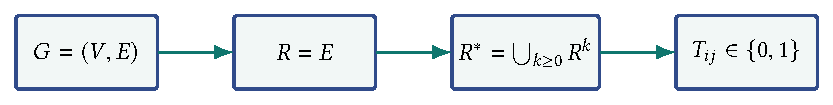
\includegraphics[width=0.82\linewidth]{figures/example-workflow.pdf}
  \caption{Illustration PDF externe et originale du déroulement de l'exemple.}
  \label{fig:external-illustration}
\end{figure}

% Remplacez le fichier et la légende. Indiquez la source et la licence de
% toute image non originale, ne déformez pas une image en imposant des
% dimensions incompatibles et contrôlez sa lisibilité à la taille
% d'impression.

\section{Équations multilignes et définition par cas}

Utilisez \texttt{align} lorsque plusieurs lignes constituent une même dérivation
et s'alignent sur un symbole pertinent. Étiquetez uniquement les lignes citées
ensuite. Par exemple,
\begin{align}
  T^{(0)}_{ij}
    &= A_{ij}\lor [i=j], \label{eq:pattern-initialisation}\\
  T^{(k)}_{ij}
    &= T^{(k-1)}_{ij}
       \lor\bigl(T^{(k-1)}_{ik}\land T^{(k-1)}_{kj}\bigr).
       \label{eq:pattern-update}
\end{align}
La mise à jour de l'\cref{eq:pattern-update} ajoute les chemins dont le nouveau
sommet intermédiaire autorisé est $k$.

Une définition par cas appartient à une équation numérotée lorsqu'elle doit être
citée :
\begin{equation}
  d(u,v)=
  \begin{cases}
    0, & u=v,\\
    \text{longueur d'un plus court chemin}, & v\text{ est accessible depuis }u,\\
    +\infty, & \text{sinon}.
  \end{cases}
  \label{eq:pattern-cases}
\end{equation}

\section{Tableau avec texte long}

Les colonnes \texttt{X} du \cref{tab:pattern-guide} partagent la largeur
disponible et renvoient automatiquement le texte à la ligne. Préférez
\texttt{tabular} pour des données numériques compactes et n'introduisez
\texttt{longtable} que si un véritable tableau doit se poursuivre sur plusieurs
pages, comme ci-dessous.

\begin{table}[htbp]
  \centering
  \caption{Choix d'une forme de tableau compacte.}
  \label{tab:pattern-guide}
  \begin{tabularx}{\linewidth}{@{}l>{\raggedright\arraybackslash}X>{\raggedright\arraybackslash}X@{}}
    \toprule
    Contenu & Traitement recommandé & Erreur fréquente \\
    \midrule
    Mesures & Indiquer unités et incertitude dans l'en-tête ou une note. & Répéter l'unité dans chaque cellule. \\
    Descriptions longues & Utiliser une colonne \texttt{X} et un texte concis. & Réduire tout le tableau jusqu'à rendre le texte illisible. \\
    Nombreuses lignes & Envisager une annexe ou un fichier lisible par machine. & Découper manuellement une ligne logique entre deux pages. \\
    \bottomrule
  \end{tabularx}
\end{table}

\section{Tableau sur plusieurs pages}

\texttt{longtable} permet à un même tableau logique de se poursuivre sur
plusieurs pages. La légende et les en-têtes de colonnes sont déclarés une seule
fois, et le bloc d'en-tête est répété sur chaque page suivante.
Le \cref{tab:pattern-checklist} montre ce schéma avec une liste de contrôle avant
dépôt.

\begin{longtable}{@{}p{0.2\linewidth}p{0.62\linewidth}c@{}}
  \caption{Liste de contrôle composée avec \texttt{longtable}.}
  \label{tab:pattern-checklist}\\
  \toprule
  Domaine & Point à vérifier & Fait \\
  \midrule
  \endfirsthead
  \toprule
  Domaine & Point à vérifier & Fait \\
  \midrule
  \endhead
  \midrule
  \multicolumn{3}{r@{}}{\emph{Suite page suivante}}\\
  \endfoot
  \bottomrule
  \endlastfoot
  Métadonnées & Titres, auteur, encadrants, année universitaire, date et mots-clés sont corrects. & $\square$ \\
  Langue & Le document principal choisi et la langue des métadonnées PDF concordent. & $\square$ \\
  Commentaires & Les commentaires de conseil (lignes commençant par \texttt{\%}) ne décrivent plus l'exemple. & $\square$ \\
  Couverture & Logos, encadrants, enseignant référent et laboratoire sont corrects et autorisés. & $\square$ \\
  Résumé & Le résumé énonce la question, la méthode, le résultat principal et les limites. & $\square$ \\
  Sommaire & Chaque chapitre et chaque annexe apparaît avec le bon numéro de page. & $\square$ \\
  Chapitres & Les chapitres d'exemple sont remplacés et aucun fichier inutile n'est inclus. & $\square$ \\
  Figures & Chaque figure est citée, légendée en dessous et lisible à l'impression. & $\square$ \\
  Tableaux & Chaque tableau est cité et légendé au-dessus, avec ses unités. & $\square$ \\
  Équations & Seules les équations citées plus loin portent une étiquette. & $\square$ \\
  Théorèmes & Les énoncés sont numérotés par chapitre et chacun est utilisé ou commenté. & $\square$ \\
  Bibliographie & Toute entrée imprimée est citée ; DOI et années ont été vérifiés. & $\square$ \\
  Liens & Renvois et citations sont résolus et aucun renvoi ne reste indéfini. & $\square$ \\
  Compilation & Une compilation complète propre ne signale ni fichier manquant ni boîte trop large. & $\square$ \\
  PDF & Les polices sont incorporées et chaque page a été relue. & $\square$ \\
  Dépôt & Le PDF final respecte les consignes du programme et de l'encadrement. & $\square$ \\
\end{longtable}

% Remplacez les lignes par votre propre tableau. Placez la légende au-dessus
% du tableau, gardez des structures de colonnes identiques pour \endfirsthead
% et \endhead, et évitez longtable pour un tableau qui tient confortablement
% sur une page.

\clearpage
\section{Code source}

Le paquet portable \texttt{listings} utilisé dans l'\cref{lst:graph-traversal}
ne demande pas de shell escape ; la coloration reste volontairement discrète.

% Pour un long programme, placez-le dans son propre fichier et chargez-le avec
% \lstinputlisting[style=TemplateCode,language=Python]{code/mon-programme.py}
\begin{lstlisting}[
  style=TemplateCode,
  language=Python,
  caption={Un court parcours de graphe.},
  label={lst:graph-traversal}
]
def reachable(graph, source):
    seen = {source}
    frontier = [source]
    while frontier:
        vertex = frontier.pop()
        for neighbor in graph.get(vertex, []):
            if neighbor not in seen:
                seen.add(neighbor)
                frontier.append(neighbor)
    return seen
\end{lstlisting}

Ensemble, ces quatre exemples
(\cref{fig:external-illustration,eq:pattern-cases,tab:pattern-guide,lst:graph-traversal})
illustrent le cycle recommandé : annoncer un objet, le présenter, lui attribuer
une étiquette stable et l'interpréter dans le texte.

    \chapter{Autres exemples LaTeX}
\label{app:more-patterns}

% Cette seconde annexe facultative rassemble d'autres formes : sous-figures,
% notation logique, unités, abréviations et page en paysage. Chaque forme
% s'appuie sur un paquet déjà chargé dans preamble.tex. Conservez ce que le
% mémoire utilise et supprimez le reste, avec son paquet.

\section{Sous-figures et flottants côte à côte}

Utilisez \texttt{subcaption} lorsque plusieurs panneaux partagent un même numéro
de figure. Chaque panneau garde sa légende, et la \cref{fig:subfigures} peut être
citée globalement ou panneau par panneau : la \cref{fig:subfigure-graph} montre
l'entrée et la \cref{fig:subfigure-workflow} le calcul.

\begin{figure}[htbp]
  \centering
  \begin{subfigure}[b]{0.46\linewidth}
    \centering
    \begin{tikzpicture}[
  vertex/.style={circle,draw=LMFINavy,thick,minimum size=8mm,inner sep=0pt},
  edge/.style={-{Stealth[length=2.4mm]},thick,LMFITeal},
  node distance=2.2cm
]
  \node[vertex] (a) {$a$};
  \node[vertex, right=of a] (b) {$b$};
  \node[vertex, right=of b] (c) {$c$};
  \node[vertex, below=1.0cm of c] (d) {$d$};

  \draw[edge] (a) -- (b);
  \draw[edge] (b) -- (c);
  \draw[edge] (c) -- (d);
  \draw[edge] (a) to[bend right=18] (d);
\end{tikzpicture}

    \caption{Graphe d'entrée.}
    \label{fig:subfigure-graph}
  \end{subfigure}\hfill
  \begin{subfigure}[b]{0.46\linewidth}
    \centering
    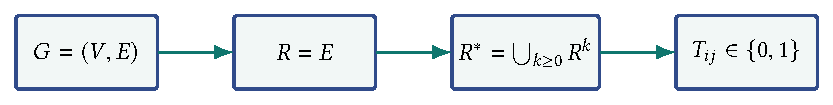
\includegraphics[width=\linewidth]{figures/example-workflow.pdf}
    \caption{Calcul.}
    \label{fig:subfigure-workflow}
  \end{subfigure}
  \caption{Deux vues de l'exemple filé.}
  \label{fig:subfigures}
\end{figure}

Une figure et un tableau peuvent aussi partager une même ligne. Placez chacun
dans une \texttt{minipage} et nommez-les avec \verb|\captionof|, comme pour la
\cref{fig:side-graph} et le \cref{tab:side-edges}.

\begin{figure}[htbp]
  \centering
  \begin{minipage}[c]{0.46\linewidth}
    \centering
    \begin{tikzpicture}[
  vertex/.style={circle,draw=LMFINavy,thick,minimum size=8mm,inner sep=0pt},
  edge/.style={-{Stealth[length=2.4mm]},thick,LMFITeal},
  node distance=2.2cm
]
  \node[vertex] (a) {$a$};
  \node[vertex, right=of a] (b) {$b$};
  \node[vertex, right=of b] (c) {$c$};
  \node[vertex, below=1.0cm of c] (d) {$d$};

  \draw[edge] (a) -- (b);
  \draw[edge] (b) -- (c);
  \draw[edge] (c) -- (d);
  \draw[edge] (a) to[bend right=18] (d);
\end{tikzpicture}

    \captionof{figure}{Le graphe d'exemple.}
    \label{fig:side-graph}
  \end{minipage}\hfill
  \begin{minipage}[c]{0.40\linewidth}
    \centering
    \begin{tabular}{cc}
      \toprule
      De & Vers \\
      \midrule
      $a$ & $b$ \\
      $b$ & $c$ \\
      $c$ & $d$ \\
      $a$ & $d$ \\
      \bottomrule
    \end{tabular}
    \captionof{table}{Sa liste d'arêtes.}
    \label{tab:side-edges}
  \end{minipage}
\end{figure}

\section{Notation logique et informatique}

Les macros du projet se trouvent dans \texttt{macros.tex} : \verb|\N|,
\verb|\Reach| et un délimiteur de crochets sémantiques \verb|\sem|. Avec elles,
\[
  \Reach(u) = \{\, v\in V \mid u\mathrel{R^*}v \,\}, \qquad
  \sem{\varphi}_G \subseteq V, \qquad
  \bigl|\Reach(u)\bigr| \leq n \in \N .
\]
Le paquet \texttt{mathpartir} compose les règles d'inférence ; voici les règles
d'introduction et d'élimination de l'implication, en style séquent :
\begin{mathpar}
  \inferrule*[right=$\to$I]{\Gamma, A \vdash B}{\Gamma \vdash A \to B}
  \and
  \inferrule*[right=$\to$E]{\Gamma \vdash A \to B \\ \Gamma \vdash A}{\Gamma \vdash B}
\end{mathpar}
Les diagrammes commutatifs utilisent \texttt{tikz-cd}. Le carré ci-dessous
commute car toute arête appartient à la clôture : les deux chemins de $E$ vers
$V\times V$ sont l'inclusion de $E$.
\[
  \begin{tikzcd}[column sep=large]
    E \arrow[r, hook] \arrow[d, hook] & R^* \arrow[d, hook] \\
    V\times V \arrow[r, equal] & V\times V
  \end{tikzcd}
\]

% Documentez dans macros.tex chaque macro de notation, et ne définissez que
% celles qui reviennent souvent. Pour les fonctions nommées, déclarez un
% opérateur (\DeclareMathOperator) plutôt que d'employer de simples lettres
% italiques.

\section{Unités, citations et notes de bas de page}

\texttt{siunitx} met en forme nombres et unités selon la langue du mémoire. La
triple boucle de l'\cref{alg:warshall} effectue \num{1073741824} mises à jour
booléennes pour $n=\num{1024}$ ; à \qty{1.5}{\giga\hertz} et une mise à jour par
cycle, cela prend environ \qty{0.72}{\second}. Les citations utilisent
\texttt{csquotes} : \enquote{une citation peut contenir \enquote{une citation
imbriquée}}, avec les guillemets de la langue active. Une note de bas de
page\footnote{Les notes de bas de page sont numérotées en continu dans un chapitre
et composées en bas de page.} reste en dehors de l'argument principal.

\section{Abréviations}

Le paquet \texttt{acro} développe une abréviation à sa première occurrence puis la
raccourcit. Un \ac{dag} n'a aucun cycle orienté, alors que chaque sommet d'une
\ac{scc} atteint tous les autres ; un \ac{dag} en est donc l'extrême opposé. Les
mentions suivantes n'emploient que \ac{dag} et \ac{scc}. Déclarez les abréviations
dans \texttt{macros.tex} ; la liste ci-dessous est produite par
\verb|\printacronyms|.

\printacronyms[heading=none]

\section{Renvois}

Écrivez \verb|\cref| au milieu d'une phrase ; \verb|\Cref| ne sert que pour commencer
une phrase par le nom de l'objet. \texttt{cleveref} ne connaît pas le genre : écrivez l'article devant le renvoi,
comme dans « la \cref{fig:subfigures} », « le \cref{tab:side-edges} », « l'\cref{alg:warshall} »
ou « de l'\cref{eq:transitive-closure} ». Plusieurs objets d'un même type peuvent
être joints : \cref{fig:subfigures,fig:side-graph}. Donnez à chaque étiquette un
préfixe court (\texttt{fig:}, \texttt{tab:}, \texttt{eq:}, \texttt{thm:}) et ne citez
que les objets dont le texte parle.

\clearpage
\begin{landscape}
\section{Un tableau large sur une page en paysage}

Un tableau trop large pour la zone de texte peut être placé sur une page tournée
avec \texttt{pdflscape} ; les visionneuses affichent la page pivotée, tout comme
la copie imprimée. Le \cref{tab:landscape} donne la taille de la matrice booléenne
et le nombre de mises à jour de la triple boucle pour des graphes de plus en plus
grands.

\begin{table}[htbp]
  \centering
  \caption{Entrées de la matrice et mises à jour booléennes de l'\cref{alg:warshall} pour $n$ sommets.}
  \label{tab:landscape}
  \small
  \begin{tabular}{@{}l *{9}{r}@{}}
    \toprule
    $n$ & \num{4} & \num{8} & \num{16} & \num{32} & \num{64} & \num{128} & \num{256} & \num{512} & \num{1024} \\
    \midrule
    Entrées $n^2$ & \num{16} & \num{64} & \num{256} & \num{1024} & \num{4096} & \num{16384} & \num{65536} & \num{262144} & \num{1048576} \\
    Mises à jour $n^3$ & \num{64} & \num{512} & \num{4096} & \num{32768} & \num{262144} & \num{2097152} & \num{16777216} & \num{134217728} & \num{1073741824} \\
    \bottomrule
  \end{tabular}
\end{table}

% N'utilisez une page en paysage que si un tableau ou une figure ne peut pas
% être rendu lisible en portrait : réduisez d'abord la police ou scindez le
% tableau. Tout objet en paysage a la même légende et le même renvoi que
% n'importe quel flottant.
\end{landscape}

  \fi
\fi
\end{document}
